\documentclass[11pt,letterpaper]{article}
\usepackage[utf8]{inputenc}
\usepackage[T1]{fontenc}
\usepackage[spanish]{babel}
\usepackage{amsmath}
\usepackage{amsfonts}
\usepackage{amssymb}
\usepackage{graphicx}
\usepackage{lmodern}
\usepackage{xspace}
\usepackage{multicol}
\usepackage{hyperref}
\usepackage{float}
\usepackage{hyperref}
\usepackage{color}

\newcommand{\azul}[1]{\textcolor{MaterialBlue900}{#1}}
\usepackage{array}

\hypersetup{colorlinks=true,   linkcolor=MaterialBlue900}
%\usepackage[colorlinks=true, linkcolor=black, urlcolor=blue, pdfborder={0 0 0}]{hyperref}

\usepackage[left=2cm,right=2cm,top=2cm,bottom=2cm]{geometry}
\title{Modelos no paramétricos y de regresión 2018-1}
\author{Tarea examen: pruebas binomiales y tablas de contingencia}
\date{Fecha de entrega: 08/01/2017}
\setlength{\parindent}{0in}
\spanishdecimal{.}


\newcommand{\X}{\mathbb{X}}
\newcommand{\x}{\mathbf{x}}
\newcommand{\Y}{\mathbf{Y}}
\newcommand{\y}{\mathbf{y}}
\newcommand{\xbarn}{\bar{x}_n}
\newcommand{\ybarn}{\bar{y}_n}
\newcommand{\paren}[1]{\left( #1 \right)}
\newcommand{\llaves}[1]{\left\lbrace #1 \right\rbrace}
\newcommand{\barra}{\,\vert\,}
\newcommand{\mP}{\mathbb{P}}
\newcommand{\mE}{\mathbb{E}}
\newcommand{\mI}{\mathbf{I}}
\newcommand{\mJ}{\mathbf{J}}
\newcommand{\mX}{\mathbf{X}}
\newcommand{\mS}{\mathbf{S}}
\newcommand{\mA}{\mathbf{A}}
\newcommand{\unos}{\boldsymbol{1}}
\newcommand{\xbarnv}{\bar{\mathbf{x}}_n}
\newcommand{\abs}[1]{\left\vert #1 \right\vert}
\newcommand{\muv}{\boldsymbol{\mu}}
\newcommand{\mcov}{\boldsymbol{\Sigma}}
\newcommand{\vbet}{\boldsymbol{\beta}}
\newcommand{\veps}{\boldsymbol{\epsilon}}
\newcommand{\mC}{\mathbf{C}}
\newcommand{\ceros}{\boldsymbol{0}}
\newcommand{\mH}{\mathbf{H}}
\newcommand{\ve}{\mathbf{e}}
\newcommand{\avec}{\mathbf{a}}
\newcommand{\res}{\textbf{RESPUESTA}\\}
\newcommand{\rojo}[1]{\textcolor{MaterialRed900}{#1}}

\newcommand{\defi}[3]{\textbf{Definición:#3}}
\newcommand{\fin}{$\blacksquare.$}
\newcommand{\finf}{\blacksquare.}
\newcommand{\tr}{\text{tr}}
\begin{document}
\begin{table}[ht]
\centering
\begin{tabular}{c}
\textbf{Maestría en Computo Estadístico}\\
\textbf{Álgebra Matricial} \\
\textbf{Tarea 2}\\
\today \\
\emph{Enrique Santibáñez Cortés}\\
Repositorio de Git: \href{https://github.com/Enriquesec/Algebra_matricial/tree/master/tareas/Tarea_2/}{Tarea 2, AM}.
\end{tabular}
\end{table}
Este documento tiene la finalidad de explicar el uso de las funciones de la tarea 2 de Algébra Matricial. 

\begin{enumerate}
\item La primera función cumple con las siguientes especificaciones:

\textit{Programe una función en r que reciba de entrada por parte del usuario el tamaño de una matriz y las entradas de la misma en orden de izquierda a derecha, de arriba a abajo. Luego, debe ir preguntando que operación elemental debe hacerse, y una vez que el usuario indique precisamente cuál, diciendo exactamente que renglones y números estarán involucrados, debe mostrarle al usuario la matriz resultante.  Cuando el usuario llegue a una forma escalonada, deberá decirle al usuario, mostrarle la matriz final y terminar el programa. Usted debe especificar al usuario cómo y en que orden debe introducir los valores y hacer las validaciones correspondientes.
}

\res
La función que realiza lo anterior esta en el archivo en R: \\$Programa1\_T2\_AM\_Enrique\_Santibáñez\_Cortés.R$.
\begin{itemize}
\item[Paso 1.] Correr todo el script completo.

\item[Paso 2.] Se solicitará el número de renglones de la matriz a ingresar. Este paso tiene una validación para solo admitir número enteros positivos, por lo que no podrá pasar al siguiente si no cumple esa condición. Dar enter para continuar. Ejemplo: Se ingresa un 2.
\begin{figure}[H]
\centering
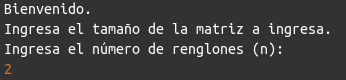
\includegraphics[scale=.7]{paso_2.png}
\end{figure}
\item[Paso 3.] Se solicitará el número de renglones de la matriz a ingresar. Este paso tiene la misma validación que el paso anterior. Dar enter para continuar. Ejemplo: Se ingresa un dos.
\begin{figure}[H]
\centering
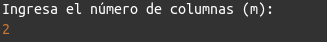
\includegraphics[scale=.7]{paso_3.png}
\end{figure}
\item[Paso 4.] Se mostrará en la pantalla el tamaño de la matriz a solicitar y empezará a solicitar los elementos de izquierda a derecha, y arriba a abajo. Se valida que solo ingrese números, de caso contrario solicitará de nuevo la entrada. Ejemplo: se agrega la matriz con los elementos: [2,3,4,5].
\begin{figure}[H]
\centering
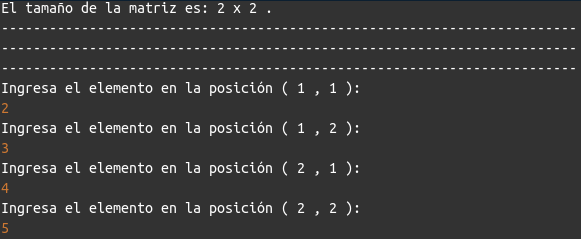
\includegraphics[scale=.7]{paso_4.png}
\end{figure}
\item[Paso 5.] Se muestra la matriz ingresada. Y se solicitara que ingrese que operación elemental se realizará:

\begin{itemize}
\item 1 para intercambiar dos renglones de la matriz (Tipo I). Se le solicitará la posición del primer vector y después del segundo vector. Ejemplo: Se intercambia el renglón 1 con el renglón 2.
\begin{figure}[H]
\centering
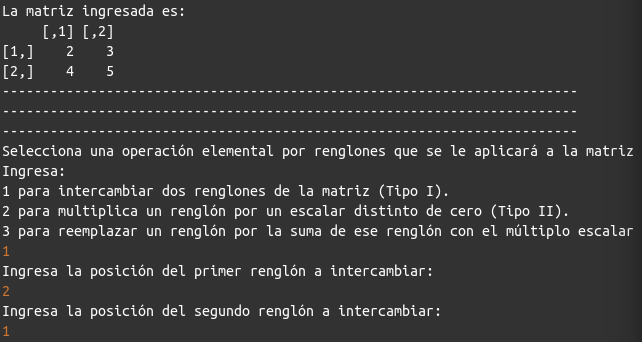
\includegraphics[scale=.7]{paso_5_11.png}
\end{figure}

\item 2 para multiplicar un renglón por un escalar distinto de cero (Tipo II). Se solicitará la posición del renglón que se le multiplicaŕa por un escalar, y después se solicitar el escalar. Ejemplo: Al renglón 1 se multiplica por 0.25.
\begin{figure}[H]
\centering
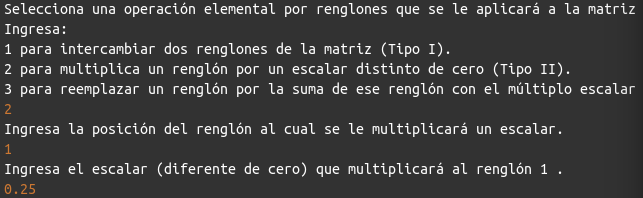
\includegraphics[scale=.7]{paso_5_21.png}
\end{figure}
\item 3 para reemplazar un renglón por la suma de ese renglón con el múltiplo escalar de otro vector. Se solicitará la posición del vector que se va a reemplazar, después la posición del segundo vector que se multiplica por un escalar y hasta último se solicita el escalar. Ejemplo: El renglón 2 se suma con el  producto de -2 por el renglón 1.
\begin{figure}[H]
\centering
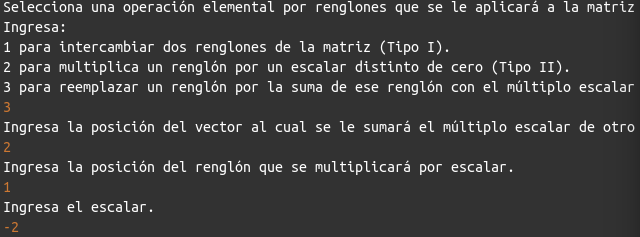
\includegraphics[scale=.7]{paso_5_23.png}
\end{figure}
\end{itemize}
\item[Paso 6.] Muestra la nueva matriz, y si verifica si esta en su forma escalonada. Si ya esta en su forma escalonada termina el programa notificando que ya la matriz esta en su forma escalonada y mostrandola. Ejemplo:
\begin{figure}[H]
\centering
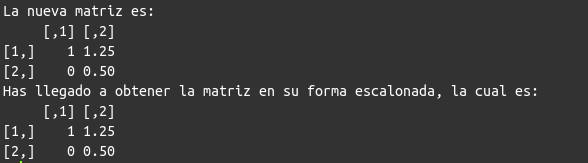
\includegraphics[scale=.7]{paso_6_1.png}
\end{figure}
\item[] Si no esta en su forma escalonada, vuelve a solicitar una nueva operación elemental y se itera desde el paso 5. Ejemplo:
\begin{figure}[H]
\centering
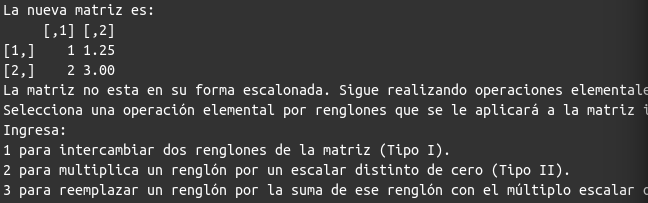
\includegraphics[scale=.7]{paso_6_2.png}
\end{figure}
\end{itemize}
\item La segunda función cumple con las siguientes especificaciones:\\
\textit{Programe una función en r que reciba de entrada una matriz y que realice la eliminación de Gauss y regrese la matriz escalonada por renglones. Es decir, a diferencia del problema 1 no debe haber intervención del usuario más que en la captura de la matriz.}

\res
La función que realiza lo anterior esta en el archivo en R:\\ $Programa2\_T2\_AM\_Enrique\_Santibáñez\_Cortés.R$.
\begin{itemize}
\item[Paso 1.] Correr todo el script completo.

\item[Paso 2.] Se solicitará el número de renglones de la matriz a ingresar. Este paso tiene una validación para solo admitir número enteros positivos, por lo que no podrá pasar al siguiente si no cumple esa condición. Dar enter para continuar. Ejemplo: Se ingresa un 2.
\begin{figure}[H]
\centering
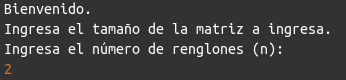
\includegraphics[scale=.7]{paso_2.png}
\end{figure}
\item[Paso 3.] Se solicitará el número de renglones de la matriz a ingresar. Este paso tiene la misma validación que el paso anterior. Dar enter para continuar. Ejemplo: Se ingresa un 2.
\begin{figure}[H]
\centering
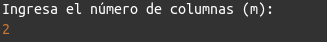
\includegraphics[scale=.7]{paso_3.png}
\end{figure}
\item[Paso 4.] Se mostrará en la pantalla el tamaño de la matriz a solicitar y empezará a solicitar los elementos de izquierda a derecha, y arriba a abajo. Se valida que solo ingrese números, de caso contrario solicitará de nuevo la entrada. Ejemplo: se agrega la matriz con los elementos: [2,3,4,5].
\begin{figure}[H]
\centering
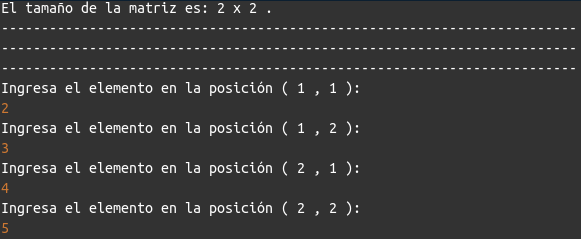
\includegraphics[scale=.7]{paso_4.png}
\end{figure}
\item[Paso 5.] Muestra la matriz ingresada y muestra la matriz en su forma escalonada y se termina la función. Ejemplo:
\begin{figure}[H]
\centering
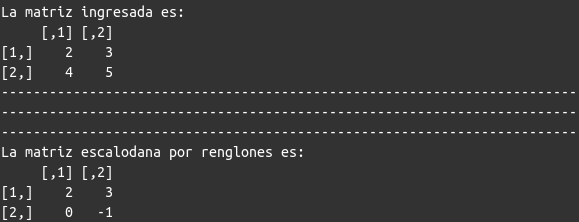
\includegraphics[scale=.7]{paso_5_2.png}
\end{figure}
\end{itemize}
\end{enumerate}

\end{document}